\documentclass{book}
\author{Sam Nolan}
\usepackage{minted}
\usepackage{graphicx}
\usepackage{listings}
\graphicspath{{images/}}
\title{Programming with ProjectX}
\begin{document}
	\maketitle
	\tableofcontents
	\chapter{Introduction}
	\section{What is ProjectX?}
	ProjectX is both a game and an educational tool for learning the basics of programming. It can be played without even touching the programming aspects as a social multiplayer game, but it becomes much more interesting when players create content of their own through the use of the programming languages Lua and XML.
	
	ProjectX is a great tool for learning programming for the first time, as it covers a wide range of skill levels. It comes with many tools that help the beginner programmer both get a feel for professional-like environments while being supported by them along the way.
	
	Professionals can also use ProjectX as just a general game. By developing on different parts of the game, every session would be completely different. If teams were to get together to mod this game, or even a classroom, the changes can be updated into one single game and can be played multiplayer by everyone. 
	
	\section{Game-Play and Rules}
	The game itself is an Real Time Strategy multiplayer game where the objective is to be the last man standing. Players connect to a server, and are spawned into an Arena. The controls are mainly touch based as the game also ports the Android and iOS platforms. Players can roam around a map with the objective of collecting resources to survive the harsh environment that they find themselves in. Players will find creatures and other features that can be interacted with. Other players can also be found and they can choose to team up or to fight, last player or team alive wins.
	
	The game imposes very few constraints about what content can be added to the game. Creature, tiles, interactions, items and much more can be added to the game to make the experience completely different. Changes that are made to the game on one device can be synced to another simply by playing on the same game.
	
	\section{Programming with ProjectX}
	ProjectX has 2 official languages, Lua and XML. These language are serve different purposes in the game. XML is used to represent objects in the game, whereas with Lua procedures can be specified. XML controls map generation, Items, Sprites and many more, whereas Lua controls Creature AI and interactions. The skills learnt can be applied to other programming languages such as Javascript, HTML or any other language that a person might want to learn.
	
	To keep things simple, what you can do is fairly limited. A programmer can only add \textit{content} to the game. That is, it is not possible to add anything that does not already exist. For instance, it is possible to create your own creature to be placed into the game, but it is not possible to add UI elements and change the rules of the game around. These are called \textit{features} and are added by the maintaining developers of the game. If you wish to see a feature in the game, you may contact Sam Nolan at NOL0055@bhs.vic.edu.au.
	
	Most of the code has its own jurisdiction, as in, the code in each folder will control only a certain aspect of the game, and no more. This is in contrast to most languages, where all code does not need to be in separate files to function. We decided to make ProjectX like this as to keep the code simple as possible.
	
	\section{Installation}
	The installation of ProjectX is reasonably straightforward. Windows is currently the only supported platform. We do have Android versions but the game is still in development and they have not been released yet. In the future, ProjectX should be supported on Linux, OSX, iOS, Android and Windows.
	
	Because the game is currently in development, receiving a copy of the game can only be done through directly asking Sam Nolan. His contact details can be found in the Developers section of Notes and Acknowledgments.  
	
	Once You have a copy of the installer (ProjectXInstall.exe), the installation is reasonably straightforward. The components that can be installed are explained below
	
	\paragraph{ProjectX}
	ProjectX is the actual game, it is required in the installation.
	
	\paragraph{ProjectX Scripting}
	The official scripting platform for ProjectX, Atom. Comes with auto-complete and error checking for scripting. It is highly recommended if developing with ProjectX.
	
	\paragraph{ProjectX Source Control}
	The Gitkraken source control package. Useful for recording and keeping changes when working in teams, not required.
	
	\paragraph{ProjectX Documentation}
	This book and the ProjectX documentation as a .chm file, which contains an official reference to everything available in ProjectX.
	
	\paragraph{ProjectX Sprite Previewer}
	A Sprite Previewer for ProjectX, This application reads a Sprite XML file  and creates sprites to preview before putting in the application. Not required but may be useful for artists.
	
	\section{Acknowledgments}
	This section concerns the developers of ProjectX, contact details are provided for some.
	
	\paragraph{Programming}
	\begin{itemize}
		\item Sam "Sparka" Nolan - NOL0055@bhs.vic.edu.au
		\item Michael Smith
	\end{itemize}
	
	\paragraph{Art}
	\begin{itemize}
		\item Oscar Taylor
		\item Adam Schembri (Codeword Gaming)
		\item Louis Evans
		\item Tom Duchemin
	\end{itemize}
	
	\paragraph{Scripting}
	\begin{itemize}
		\item Hung Dao
	\end{itemize}
	
	\paragraph{Music}
	\begin{itemize}
		\item Louis Evans
	\end{itemize}
	
	\chapter{Developing With ProjectX}
	This section addresses the structure of ProjectX and how to use some of the tools that come with it.
	
	\section{Structure of ProjectX}
	All the ProjectX source files can be found in Local AppData for Windows, that is, \texttt{C:\textbackslash Users\textbackslash [Username]\textbackslash AppData\textbackslash Local\textbackslash ProjectX} The AppData folder is hidden, so you may need to enable seeing hidden files.
	
	This folder can also be accessed by opening it with Atom. The ProjectX Scripting link will automatically direct to the resources folder.
	
	\section{Atom}
	Atom is the official scripting platform for ProjectX. The actual Atom project can be found at \texttt{atom.io}. There is a package (or extension) to Atom which contains error checking and code-completion for ProjectX. The package is installed with Atom from the installer.
	
	\chapter{ProjectX XML}
	\section{Beginning With XML}
	XML is called a \textbf{markup language}. A markup language has a certain syntax that uses angle brackets and tags. It is nearly identical to HTML in syntax. This is an example of a tag:
	
	\begin{center}
		\texttt{<class>}
	\end{center}
	
	What makes it a tag is the angle brackets around it, "class" is the \textbf{name} of the tag. In ProjectX there are many different tags that are differentiated by name that have a variety of uses. For example the \texttt{<class>} tag is used in the players XML file to specify a character class.
	
	Every tag has a matching ending tag. The ending tag is the same as the original (starting) tag except that it starts with a forward slash (/)

	\begin{center}
		\texttt{</class>}
	\end{center}
	
	Anything between the ending tag and the original starting tag is said to be inside the tag, for example:
	\begin{minted}[tabsize = 4]{xml}
<description>
	This is a description!
</description>
	\end{minted}
	The "This is a description!" is said to be the description tag's value. We can have tags inside tags like so:
	\begin{minted}[tabsize = 4]{xml}
<class>
	<description>
		This is a description!
	</description>
</class>
	\end{minted}
	The description is inside the class and the text is inside the description. You can make many different structures using XML.
	
	In XML, any tag can have \textbf{attributes} associated with it. An attribute looks like this:
	\begin{minted}[tabsize = 4]{xml}
<class name="Rat Man">
	
</class>
	\end{minted}
	In this case, \texttt{name} is an attribute of the \texttt{class} tag. and the \textbf{value} of the name attribute is \texttt{"Rat Man"}. In ProjectX, all attribute values are surrounded by quotes. The quotes are not part of the value, but just group the text in between them together. This is called a \textbf{string} and comes in various programming languages. For example, the string \texttt{"Hello World!"} represents the literal value of \texttt{Hello World!}.
	
	That concludes the basics of XML. The following sections show how XML can be used in different areas of the game. It is in order of the easiest things to learn to the hardest.
	
	\section{Sprites}
	The sprites XML file is not necessarily the easiest to learn but is required by the other scripts.

	The sprites XML file contains all the different sprites that will be used in various other aspects of the game, those aspects being players, tiles, creatures and items. Here is an example of a sprites XML file.

\begin{minted}[tabsize = 4]{xml}
<items>
	<spritesheet source = "Resources.png" >
		<sprite name="Gold" x="0" y="0" />
		<sprite name="Wood" x="1" y="0" />
		<sprite name="Stone" x="2" y="0" />
		<sprite name="Apple" x="3" y="0" />
	</spritesheet>

	<spritesheet source="StandardTools.png" >
		<sprite name="Pickaxe" x="0" y="0" />
		<sprite name="Shovel" x="1" y="0" />
		<sprite name="Sword" x="0" y="1" />
		<sprite name="Axe" x="1" y="1" />
	</spritesheet>

	<spritesheet source="Ultanium.png" >
		<sprite name="Ultanium" x="0" y="0" />
	</spritesheet>

	<spritesheet source = "UltaniumGodbladeAni.png">
		<animate name="Ultanium Godblade" height="6" width = "1" x="0" y="0" speed="0.08" />
	</spritesheet>

</items>

<tiles>
	<spritesheet source = "terrain.png" tileWidth= "1" tileHeight = "1" >
		<sprite name="water" x ="0" y="0" />
		<sprite name="sand" x="1" y="0" />
		<sprite name="grass" x="2" y="0" />
		<sprite name="cliff" x ="0" y ="1" />
		<sprite name="stoneFloor" x ="3" y="0" />
		<sprite name="snow" x = "1" y="1" />
		<sprite name="graveStoneFloor" x="2" y="1" />
		<sprite name="graveGrass" x="3" y="1" />
	</spritesheet>

	<spritesheet source="graveMisc.png" tileWidth="1" tileHeight="2" >
		<sprite name="grave-deadTree" x = "0" y = "0" />
		<sprite name="grave-gravestone" x = "1" y = "0" />
		<sprite name="grave-spookyStatue" x = "2" y = "0" />
	</spritesheet>

	<spritesheet source = "tree.png" tileWidth = "1" tileHeight = "3" >
		<sprite name="tree" x="0" y = "0" />
	</spritesheet>

	<spritesheet source = "misc.png" tileWidth = "1" tileHeight = "1" >
		<sprite name="coal" x="0" y = "1" />
		<sprite name="mudrock" x = "1"  y="1" />
		<sprite name="coal2" x = "0" y = "0" />
		<sprite name="gold" x = "1" y = "0" />
	</spritesheet>

	<spritesheet source="Small Trees.png" tileWidth = "1" tileHeight = "2" >
		<sprite name="palm" x="0" y="0" />
		<sprite name="cactus" x="1" y="0" />
		<sprite name="shrubbery" x="0" y="1" />
		<sprite name="appleTree" x="1" y="1" />
	</spritesheet>
	<spritesheet source="Supertall Tree.png" tileWidth = "1" tileHeight ="4" >
		<sprite name="SuperTreh" x="0" y="0" />
	</spritesheet>

	<spritesheet source="Eggstoudanry_Statue.png" tileWidth = "1" tileHeight = "2">
		<sprite name="eggStatue" x="0" y="0" />
	</spritesheet>
	<spritesheet source="deadlands.png" tileWidth = "1" tileHeight = "1">
		<sprite name="deadlandsFloor" x="0" y="0" />
	</spritesheet>
</tiles>

<creatures>
	<spritesheet source= "Rat anim.png" height= "10" width="16">
		<animate name="Rat Left" height="6" width= "1" x="0" y="0" speed="0.1" />
		<animate name="Rat Right" height="6" width= "1" x="1" y="0" speed="0.1" />
		<sprite name="Rat Left Idle" x="0" y="0" />
		<sprite name="Rat Right Idle" x="1" y="0" />
	</spritesheet>

	<spritesheet source= "BigRatAnim.png" height="13" width="17">
		<animate name="Big Rat Left" height="6" width="1" x="0" y="0" speed="0.1" />
		<animate name="Big Rat Right" height="6" width="1" x="1" y="0" speed="0.1" />
		<sprite name="Big Rat Left Idle" x="0" y="6" />
		<sprite name="Big Rat Right Idle" x="1" y="6" />
	</spritesheet>
</creatures>

<players>
	<spritesheet source="Birdfoot.png" height="30" width="15">
		<sprite name="Birdfoot" x="0" y="0" />
	</spritesheet>
	<spritesheet source="Hot Dog Man.png" height="29" width= "20">
		<sprite name="Hot Dog Man" x="0" y="0" />
	</spritesheet>

	<spritesheet source = "BigRatAnim.png" height="13" width="17">
		<animate name="Rat Man Left" height="6" width="1" x="0" y="0" speed="0.1" />
		<animate name="Rat Man Right" height="6" width="1" x="1" y="0" speed="0.1" />
		<sprite name="Rat Man Left Idle" x="0" y="6" />
		<sprite name="Rat Man Right Idle" x="1" y="6" />
	</spritesheet>
</players>
\end{minted}
	As you can see, the sprites XML file is split up into sections, those sections being \texttt{<creatures> <players> <tiles>} and \texttt{<items>}. This section seperate the different places where the sprites will be used in the game.

Inside each of these sections are spritesheets, these spritesheets correspond to different files inside the res/sprites folder. Here is a listing of the res/sprites:

\begin{lstlisting}
res/sprites
├── creatures
│   ├── BigRatAnim.png
│   ├── Rat anim.png
├── items
│   ├── Resources.png
│   ├── UltaniumGodbladeAni.png
│   ├── Ultanium.png
├── players
│   ├── BigRatAnim.png
│   ├── Birdfoot.png
│   └── Hot Dog Man.png
└── tiles
    ├── deadlands.png
    ├── Eggstoudanry_Statue.png
    ├── graveMisc.png
    ├── misc.png
    ├── Small Trees.png
    ├── Supertall Tree.png
    ├── terrain.png
    └── tree.png
\end{lstlisting}

The source attribute of the spritesheet tag tells the game where to find the image file. As the folder struvture suggests, the sections are split up into their own folders, for organisation. Other than the source attribute, the attributes for the spritesheet tag are different for all the different sections, this is because the size of some sprites can be inferred from their context. Items will always be 32x32, while tiles will be in lots of 32 and 24 (width and height respectively). 

Because of this, spritesheets have different attributes for width and height depending on their section, the attributes are as follows:

\paragraph{items} No extra attributes needed, sprites are assumed to be 32x32.
\paragraph{tiles} \texttt{tileWidth} and \texttt{tileHeight} are measured in tiles and outline the tiles size, for width, it is in lots of 32 pixels, for height, it is in lots of 24 pixels
\paragraph{creatures and players} \texttt{height} and \texttt{width} attributes are measured in pixels.

The spritesheet contains many sprites within it, each sprite must be the same size inside the spritesheet. The sprites inside the spritesheet can be specified with the \texttt{sprite} or \texttt{animate} tag. The different between the two is that a sprite is a static image whereas the animate moves and flicks through frames and creates an animation. It is highly reccomended that you make animations for players and creatures, tiles and items are acceptable to not be animated.

The sprite tag has a \texttt{name, x} and \texttt{y} attribute. The name is the name of the sprite inside the spritesheet for use later. With items and tiles, this name must correspond with the exact name of the item/tile in the their respective XML files. With creatures and players, it is possible (and reccomended) to have multiple sprites associated with on entity. For example there may be a sprite of the creature going right and another of the creature going left. This means that the name of the sprite does not need to match the name of the creature of player, but it should resemble it in some way for clarity.

The \texttt{x} and \texttt{y} attributes specify where the sprite is found on the tilesheet. They start in the top left and move down to the bottom right. For example, consider the image below:

\begin{figure}[ht!]
		\centering
		
\includegraphics[width=90mm]{terrain.png}
		\caption{Sample spritesheet}
\end{figure}

This image contains various floor types, the corresponding spritesheet tag for this spritesheet is as follows:

\begin{minted}[tabsize = 4]{xml}
<spritesheet source = "terrain.png" tileWidth= "1" tileHeight = "1" >
		<sprite name="water" x ="0" y="0" />
		<sprite name="sand" x="1" y="0" />
		<sprite name="grass" x="2" y="0" />
		<sprite name="cliff" x ="0" y ="1" />
		<sprite name="stoneFloor" x ="3" y="0" />
		<sprite name="snow" x = "1" y="1" />
		<sprite name="graveStoneFloor" x="2" y="1" />
		<sprite name="graveGrass" x="3" y="1" />
</spritesheet>
\end{minted}

The animate tag has a few more attributes, to illustrate, We will use the example of the Big Rat. This is the xml for the sprite:
\begin{minted}[tabsize = 4]{xml}
<spritesheet source= "BigRatAnim.png" height="13" width="17">
		<animate name="Big Rat Left" height="6" width="1" x="0" y="0" speed="0.1" />
		<animate name="Big Rat Right" height="6" width="1" x="1" y="0" speed="0.1" />
		<sprite name="Big Rat Left Idle" x="0" y="6" />
		<sprite name="Big Rat Right Idle" x="1" y="6" />
</spritesheet>
\end{minted}

\begin{figure}[ht!]
		\centering
		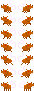
\includegraphics[width=40mm]{BigRatAnim.png}
		\caption{Big Rat animation}
\end{figure}

That attributes for tha nimate tag are a bit more complicatated. the x and y attributes are which sprite the animation starts on, the height attribute is how vertically sized the attribute is. In this case the animation is 6 high because there are 6 sprites that are above each other which willbe cycled through. The width is similar. Currently, the animation will run in a top-down left to right order. The speed is how many seconds each sprite should be displayed, in this instance, a sprite is only shown for a tenth of a second.

With this example, there are also normal sprites inside the spritesheet, it is possible to mix animates and sprites in the same spritesheet, it is also possible to have animates and sprites sharing sprites, like the (small) rat example above.

Even though there are no animations for tiles currently, it is entirely possible to do so.

\section{Music}
The support for the music in XML is trivial, and it may be removed in the future as it can be done through Lua. But nevertheless, the music XML file is one of the simplest XML files to learn, here is an example of the music xml file:
\begin{minted}[tabsize = 4]{xml}
<region name="plains">
	<song source="Ambient Hope" />
</region>
<region name="snow">
	<song source="Chase in the cold" />
</region>
<region name="beach">
	<song source="Seaside" />
</region>
<region name="graves">
    <song source="Ambient Despair" />
</region>
<region name="cliffs">
	<song source="Grind" />
</region>
<region name="desert">
	<song source="A little warm" />
</region>
\end{minted}

If you think that you understand how this works, you probably do. The region tag is a region of tiles as specified in the map generation XML file. The \texttt{name} attribute is the name of the region. The song tag is the song to be played in that region, and the source is the name of the song to be played. The music can be found in res/music. The current listing of this file is as below:

\begin{lstlisting}
res/music
├── A chase!.wav
├── A little warm.wav
├── Ambient Despair.wav
├── Ambient Hope.wav
├── Ambient Nostalgia.wav
├── Chase in the cold.wav
├── Endgame.wav
├── Grind.wav
├── In the grime.wav
├── My Song 4.wav
├── Rust.wav
├── The Vain King.wav
└── Transformation.wav
0 directories, 13 files
\end{lstlisting}

As you can see, you do not need to include the file extension with the source name. Also, there are many tracks that have not been added to the game yet.

The music XML file may be improved on in the future.

\section{Items}
The Items XML file contains all the things that can be picked up and placed inside your inventory, here is a sample of the Items XML file:

\begin{minted}[tabsize = 4]{xml}
<item name="Pickaxe">
	<ingredients>
	Wood:3;
	Stone:3;
	</ingredients>
	<description>
	Tired of smashing a rock with wood?
Now you can do the same... with stone!
	</description>
</item>

<item name="Shovel">
	<ingredients>
	Wood:3;
	Stone:1;
	</ingredients>
	<description>
	For when your hands just aren't enough.
	</description>
</item>

<item name="Axe">
	<ingredients>
	Wood:3;
	Stone:2;
	</ingredients>
	<description>
	Got wood? Now you do! 
Well... soon, at least.
	</description>
</item>

<item name="Sword">
	<ingredients>
	Wood:1;
	Stone:3;
	</ingredients>
	<description>
	For killing the good... and the bad...
and the mediocre.
	</description>
</item>
\end{minted}

These are the basic tools found in ProjectX, the Pickaxe, Shovel, Axe and Sword. The name attribute is the display name of the item and also the exact name of the sprite that will be displayed with the item.

The item tag can have 2 children, the first is the ingredients tag, the tag includes what is needed to craft the item. The ingredients tag is not neccesary and the item can be obtained through other ways (like getting it through a lua script). The syntax for the ingredients is simple:

\begin{center}
		\texttt{[item] : [quantity] ;}
\end{center}

Make sure to include the semicolon at the end of the ingredient, it seperates them. For example, the statement \texttt{Wood:3;Stone:1;} is perfectly legal, but is not reccomended for legability reasons.

It is possible to have multiple recipies for items, meaning that the item will become craftable when any of the recipies are furfilled.

The other tag inside the item tag is the description, this is text that is shown with the item, there is a theme of sattire with these descriptions.

\section{Interactions}
The interactions XML file tells the game what to do when different items are clicked on around the map, here is an example of the interactions XML file:

\begin{minted}[tabsize = 4]{xml}
<movable>
	sand;cliff;snow;graveGrass;graveStoneFloor;deadlandsFloor;grass
</movable>
<tile name="gold">
	<action>giveAndDestroy("Gold", 3)</action>
</tile>

<tile name="coal">
	<action>giveAndDestroy("Stone", 3)</action>
</tile>

<tile name="tree">
	<action>giveAndDestroy("Wood", 3)</action>
</tile>

<tile name="grave-deadTree">
	<action>giveAndDestroy("Wood", 3)</action>
</tile>

<tile name="appleTree">
	<action name="chop">giveAndDestroy("Wood", 3)</action>
	<action name="pick">inventory:giveItem("Apple")</action>
</tile>
\end{minted}

The file consists of \texttt{tile} tags. Each tag represents an tile specified in the map generation XML file. The name attribute is the exact name of the tile. Each tile can have one or more actions assosiated with it. The text inside the action tag is Lua code that will be excecuted after the player has clicked and walked to the tile. In this case, clicking on the gold tile will cause the player to walk up to the gold tile and destroy it, giving is 3 gold in the process. The function \texttt{giveAndDestroy} is a custom one and not part of the standard functions, more information on this can be found at the Lua interactions section. If there is more than one action available, the user will be prompted for which action they would like to do.

\begin{figure}[ht!]
		\centering
		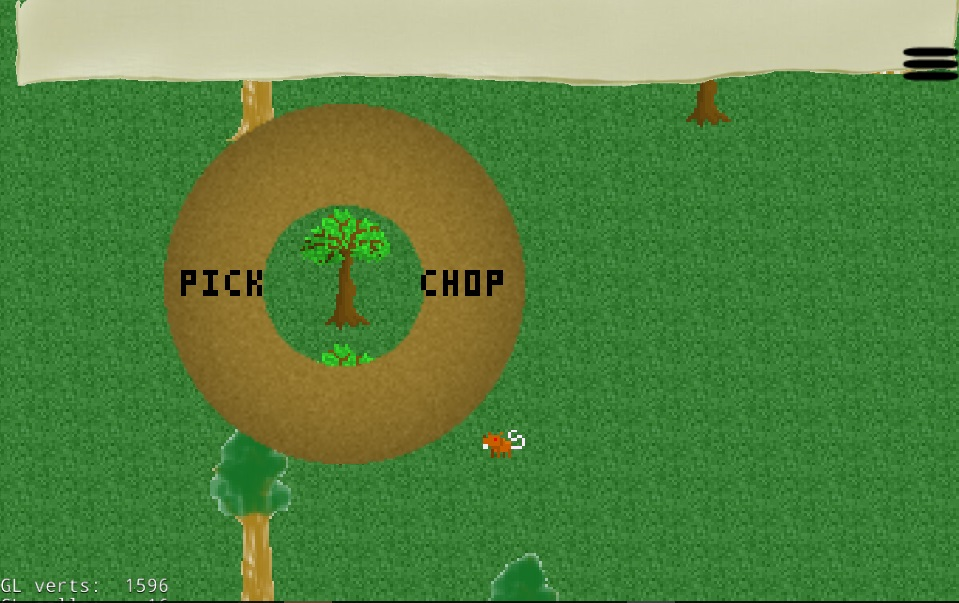
\includegraphics[width=90mm]{MultipleSelection.jpg}
		\caption{Selection Wheel}
\end{figure}

If there is no choice, the \texttt{name} attribute of the action is not needed as it is never shown. The lua code is run in the \textbf{interactions} scope.

The movable tag at the top is for convenience, this tag lists all the tiles, seperated by semicolons, that can be walked on.

\section{Players}
The Players XML file is where all the playable character classes are listed. Here is an example of the file:

\begin{minted}[tabsize = 4]{xml}
<class name="Birdfoot">
	<movement>
		<leftIdle>Birdfoot</leftIdle>
		<rightIdle>Birdfoot</rightIdle>
		<left>Birdfoot</left>
		<right>Birdfoot</right>
	</movement>
	<description>
	Birdfoot is coolz
	</description>
</class>

<class name="Rat Man">
	<movement>
		<leftIdle>Rat Man Left Idle</leftIdle>
		<rightIdle>Rat Man Right Idle</rightIdle>
		<left>Rat Man Left</left>
		<right>Rat Man Right</right>
	</movement>
	<description>
	I do it 4 da cheez
	</description>
</class>
\end{minted}

The \texttt{class} tag is a single character class that can be played as. the \texttt{name} attribute is the display name of the class.

The class tag has 2 children, those being the \texttt{movement} tag and the \texttt{description} tag. The movement tag is the same as the creature movement tag, and has 16 possible children, being \texttt{<left> <right> <up> <down> <upLeft> <upRight> <downLeft> <downRight> <leftIdle> <rightIdle> <upIdle> <downIdle> <upLeftIdle> <upRightIdle> <downLeftIdle>} and \texttt{<downRightIdle>}, which contain the name of the sprite or animation that will be played when the character is in that position. Movements must be given for at least left, right, left-idle and right-idle the rest can be inferred but the more directions the better.

The description tag is a written description shown beside the player.

Birdfoot is a good example of a bad character class. This is because all the sprite directions and the same sprite, giving the impression that the player is riding a segway, it may be included in the future that players without animation when moving will ride segways.

\begin{figure}[ht!]
		\centering
		
\includegraphics[width=40mm]{Nice_Segway.png}
		\caption{Future Segway sprite}
\end{figure}

\section{Creatures}
The creatures XML file contains creatures that can be spawned into the game, here is an example of the creatures XML file:

\begin{minted}[tabsize = 4]{xml}
<creature name="Rat" ai="Rat" speed="2">
	<movement>
		<left>Rat Left</left>
		<right>Rat Right</right>
		<leftIdle>Rat Left Idle</leftIdle>
		<rightIdle>Rat Right Idle</rightIdle>
	</movement>
</creature>

<creature name="Big Rat" ai="Rat" speed="3">
	<movement>
		<left>Big Rat Left</left>
		<right>Big Rat Right</right>
		<leftIdle>Big Rat Left Idle</leftIdle>
		<rightIdle>Big Rat Right Idle</rightIdle>
	</movement>
</creature>
\end{minted}

The \texttt{creature} tag has 3 known attributes, the first is the name, which is the name of the creature so that it can be referenced when spawning it in lua. The \texttt{ai} attribute contains the filename of the lua file that will be used to be it's ai, without the \texttt{.lua} extension. These AI scripts can be found in \texttt{script/lua/creatures}. The speed attribute is how fast the creature can move in tiles per second.

The only known child of the creature tag is the movement tag, which is the same as the players XML movement tag, please see that section for a reference on it.

\section{Map generation}
Map generation was the first XML file to be added to the game and is by far the most complicated. Here is an example of the Map generation XML file:

\begin{minted}[tabsize = 4]{xml}
<map width="1500" height="1500" name="standard">
	<layer name="bottom">
		<rule type="perlin" scale="0.2">
			<tile name='water' height="20"/>
			<tile region='beach' name='sand' height="24" />
			<area height="70">
				<tile region='plains' name='grass' />
				<rule type="perlin" scale="0.5">
					<tile region='deadlands' name='deadlandsFloor' height="10" />
				</rule>
				<rule type="perlin" scale="0.5">
					<tile region='desert' name="sand" height="10" />
				</rule>
				<rule type="perlin" scale="0.5">
					<rule region='graves' type="random" height="10">
						<tile name='graveStoneFloor' height="95" />
						<tile region='graveDirt' name='graveGrass' height="100"/>
					</rule>
				</rule>
			</area>
			<tile region="cliffs" name='cliff' height="90" />
			<tile region='snow' name='snow' height="100" />
		</rule>
	</layer>
	<layer name="misc">
		<rule type="inside" inside="desert" >
			<rule type="random">
				<tile name="cactus" height="1" />
			</rule>
		</rule>
		<rule type="inside" inside="plains">
			<rule type="random">
				<tile name="SuperTreh" height = "0.1" />
				<tile name="tree" height = "2" />
				<tile name="appleTree" height="3" />
			</rule>
		</rule>
		<rule type="inside" inside="cliffs">
			<rule type="random">
				<tile name="coal" height ="2"/>
				<tile name="mudrock" height ="5" />
				<tile name="coal2" height = "7"  />
				<tile name="gold" height = "10"  />
			</rule>
		</rule>
		<rule type="inside" inside="beach">
			<rule type="random">
				<tile name="palm" height ="2" />
			</rule>
		</rule>
		<rule type="inside" inside="graves">
			<rule type="random">
				<tile name="grave-gravestone" height = "2" />
				<tile name="grave-spookyStatue" height = "2.4" />
			</rule>
		</rule>
		<rule type="inside" inside="graveDirt">
			<rule type="random">
				<tile name="grave-deadTree" height = "50"  />
			</rule>
		</rule>
		<rule type="inside" inside="deadlands">
			<rule type="random">
				<tile name="eggStatue" height = "4" />
			</rule>
		</rule>
	</layer>
</map>
\end{minted}

As you can see, this file is much more complicated than all the other XML files, but is still reasonably easy to learn. Lets start from the top

First of all, there is the \texttt{map} tag. This tag contains the map generation rules. It is possible to have multiple map generation techniques (This one is called "standard") and the player can select what map they would like to play. The \texttt{name} attribute is the display name of the map generation technique. The \texttt{height} and \texttt{width} attributes are how many tiles wide and high the map is, even though there is no performance issues with generating large maps, generating maps larger than 32,000 tiles wide/high will cause issues. The size of 1,500 is rather large and takes about 9 minutes to walk across.

Next up there is the layer tag, there are 2 layers, the bottom layer and the misc layer. The bottom layer contains all the floor tiles, where the top layer contains all the things placed on top of those tiles. The layers do not actually need the name attribute, but is here for illustrative purposes.

Now we get into map generation rules. A map generation rule tells how it's child rules and tiles are placed, there are 2 types of tags for rules, \texttt{rule} and \texttt{area}. They behave differently.

The rule tag gives every tile on the map a value from 0-100, or a \textbf{height}. Then, all of it's children have a hieght also, and the height of the tile is compared with the height of the rule to determine whether it should be placed. 


\begin{figure}[ht!]
		\centering
		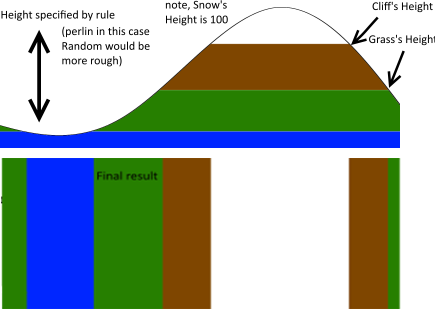
\includegraphics[width=90mm]{MapGenRules.png}
		\caption{Map rules example}
\end{figure}

If the height specified by the tile is higher than the one generated by the rule, the tile will be placed.

The XML for the diagram could be this:
\begin{minted}[tabsize = 4]{xml}
<rule type="perlin" scale="0.2">
	<tile name="water" height="20" />
	<tile name="grass" height="60" />
	<tile name="cliff" height="80" />
	<tile name="snow" height="100" />
</rule>
\end{minted}

In the example above, lets say that the height generated for a certain tile is 56. Because 20 is smaller than 56, the water tile will not be placed. But grass has a height of 60 and is higher than 56 and therefore will be placed. Notice how 80 and 100 are both higher than 56 but are not placed as grass is a closer match.

These can also be thought of as percentages. This configuration has water appearing 20\% of the time, grass 40\%, cliff 20\% and snow 20\%.

The value that the rule gives can vary to acheive different effects. The example above uses a "perlin" rule as the values smoothly change, making the possibility for hills and valleys and similar tiles to be placed together. 

These different rules are \textbf{types} of rules. There are 3 types of rules, perlin, random and inside. The examples below show how the rule choses it's heights.

\begin{figure}[ht!]
		\centering
		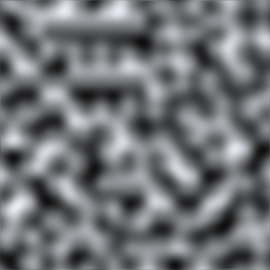
\includegraphics[width=90mm]{PerlinNoiseExample.png}
		\caption{Perlin Noise}
\end{figure}


\begin{figure}[ht!]
		\centering
		
\includegraphics[width=90mm]{WhiteNoiseExample.png}
		\caption{White Noise}
\end{figure}

Perlin noise's size can be changed with a \texttt{scale} attribute. The smaller the scale, the more zoomed out. The larger the scale, the closer it comes to white noise.

The final rule type is inside, which will always place it's children if it inside a certain \textbf{region}. These may only be used on the second layer (misc).

All tiles and rules can have regions associated with them. A region is a group of tiles that are singled out for any particular reason. Regions can be used to play music when a player moves into them, or they may have things placed in the second layer that only appear \textit{inside} a certain region. Regions can also be found through Lua.

Many examples of the inside rule can be found in the large example above.

The area tag behaves a bit differently to the rule tag, it places tiles by putting the tiles in layers. The first child inside the area tag is placed first, then the second child will be placed in top, and so on. This means that the layer above the first should have places where there are no tags placed. For example:

\begin{minted}[tabsize = 4]{xml}
<rule type="perlin" scale="0.2">
	<tile name="water" height="20" />
	<tile name="grass" height="60" />
</rule>
\end{minted}

Here, no tiles will be placed if the height generated by the rule is larger than 60, leaving holes in this layer so the layer below can be shown. This is useful for adding biomes, anything you can do with the area tag is possible with the rule tag, it is only there for convenience.

Finally, the tile tag is a single sprite for a tile. The \texttt{name} attribute of the tile is the name of the sprite in the sprites XML.

\chapter{ProjectX Lua}
\section{Begginning with Lua}
Lua is the other language that is used often in the game. Lua differs from XML because it is a \textbf{procedual} language. This means that instead of writing about objects like you would in XML, as it is a \textbf{markup} langauge, you write about procedures, that is, how to do things. Lua controls what happens at the start of the game, how creatures behave and what happens when you interact with tiles.

\subsection{Functions}

A basic Lua program might look like this:
\begin{minted}[tabsize = 4]{lua}
Debug.log("Hello world");
\end{minted}

This prints \texttt{Hello world} to the console, and the log file. Lets break this program down.

\texttt{Debug.log} is called a \textbf{function}. A function simply does something, in this case, the function \texttt{Debug.log} logs a message. The matching brackets after the function hold what are called the \textbf{arguments}. \texttt{"Hello world"} is the argument to \texttt{Debug.log}. Arguments are values that are given to the \textbf{function} to tell it how to act. We want \texttt{Debug.log} to print the value \texttt{Hello world} so we gave it the value to print. Arguments appear elsewhere in many other functions. For example, \texttt{Music.playSong} takes an argument which tells it what song to play, for example: \texttt{Music.playSong("Enter the dungeon");}. The quotes around \texttt{Hello world} turns the value into a \textbf{string}. A string could be a word, a sentence, or an Epic poem, as long as it contains letters in it. The quotes make it pass the \textbf{literal} Hello world to the function. Finally the semicolon finishes the line. It is worth noting that you do not need to place the semicolon in Lua, although it is good practise because many other languages end there lines with a semicolon.

Here are a few other example of function calls:
\begin{minted}[tabsize = 4]{lua}
Debug.logWarning("Don't spill the milk");
Music.playRegionSong("cliff");
Player.getByIndex(0);
\end{minted}

Functions can have multiple arguments, those arguments are seperated by semicolons. For example, often it is needed to specify what tile you want the function to affect, so you can supply an x and y value for which tile you are talking about. \texttt{Particles.spawnParticles("fire", 78, 103);} is an example of a function with 3 arguments, a name, an x coordinte, and a y coordinate.

\subsection{Types}

In lua, there are different \textbf{types} of values. We have already seen some of them.

\paragraph{string}
A very common type is a string, a string is a list of characters, for example "Fire" is a string, or "Enter the Dungeon", or even "4". As you can see, strings are denoted by quotes around the value, the quotes mean "I am talking about the actual text between the quotes", that sentence there could be a string.

\paragraph{number}
A number is exactly what it sounds like. 2, 8.7, 1089 and -8.9 are all numbers

\paragraph{table}
A table is another very useful type. A table is a collection of things, if you have worked in other languages, the table is similar to an \textit{array} or \textit{list}. For example, you can have a table of lottery numbers, if your lottery number are 12, 35 and 62, then the table would be written like \texttt{\{12,35,62\}}. Tables are bery useful for keeping related information together.

\subsection{Variables}
A variable is simply a stored piece of information. This information is given a name and it can then be used later in the program and changed. To start with a variable, you must first declare it, for example:

\begin{minted}[tabsize = 4]{lua}
myDJName = "DJ Steve";
songCount = 8;
salary = 0.10;
phoneNumbers = {5719349537, 724236216};
\end{minted}

All these values can be used later in the program with the name that you gave them.

\begin{minted}[tabsize = 4]{lua}
Debug.log(myDJName);
\end{minted}

Accessing values of tables is an interesting case, for example, if you wanted to get the first value or the phone numbers, you would use:

\begin{minted}[tabsize = 4]{lua}
phoneNumbers[1]
\end{minted}


\end{document}
